\section{Preliminaries}
\label{Prelims}

\subsection{Notation}

First we introduce notation for expressing graph metrics. This notation will also be used throughout the paper. % TODO - GET RID OF SECOND LINE?

\begin{definition}
	Complement Set

	\noindent
	Given a graph $G = (V, E)$, for a set of vertices $S \subseteq V$ we define the complement set $\comp{S} = V \setminus S$
\end{definition}

\begin{definition}
	Cut Set

	\noindent
	Given a graph $G = (V, E)$, for a set of vertices $S \subseteq V$ we define the cut set $ E(S, \comp{S}) = \left\{\{u, v\} \in E \mid u \in S, v \in \comp{S} \right\}.$
\end{definition}

\begin{definition}
	Degree of a vertex

	\noindent
	Given a graph $G = (V, E)$, let $d_v$ be the number of neighbouring nodes $v$ is adjacent to, i.e. $$
		d_v = |\left\{ e \in E : v \in e \right\}|
	$$
\end{definition}

\begin{definition}
	Volume of a vertex set

	\noindent
	Given a graph $G = (V, E)$ with $S \subseteq V$, let 
	$$
		\text{vol}(S) = \sum_{v \in S} d_v
	$$
\end{definition}

% TODO: Explain Implications of Cut set defn?

\subsection{Graph Metrics}\label{subsect:graphMetrics}

\begin{definition}
	Conductance of a graph $G = (V, E)$
	$$
		\Phi(G) = \min_{\emptyset \neq S \subset V} \frac{|E(S, \comp{S})|}{\min\{\text{vol}(S), \text{vol}(\comp{S})\}}
	$$
\end{definition}

\begin{definition}
	Diligence of a cut $ E(S, \comp{S}) $
	$$
		\rho(S) = \comp{d}(S) \min_{\{u, v\} \in E(S, \comp{S}) } \left\{ \max \left\{ \frac{1}{d_u},\frac{1}{d_v} \right\} \right\}
	$$ 
	where $\comp{d}(S) := \frac{\sum_{v \in S} d_v}{|S|}$ is the average degree of the vertices in $S$
\end{definition}

\begin{definition} % TODO: This definition doesn't include size bounds on S
	Diligence of a graph $G$
	$$
		\rho(G) = \min_{0 < \text{vol}(S) \leq \frac{\text{vol}(V)}{2}} \rho(S) 
	$$
\end{definition}

\subsection{Introducing Dynamic Networks}

Here we formally define the Dynamic Network structure rumours will spread on.

\begin{definition}
	Dynamic Network

	\noindent
	A dynamic network is a sequence of graphs $\mathcal{G} = (G_t)_{t \in \mathbb{N}}$ indexed by an integer time $t$. All the graphs in the sequence have the same vertex set at each time step, but the edge set may vary, i.e.  $G_t = (V, E_t)$ where $E_t$ is some edge set on $V$.
\end{definition}

$G_t$ represents the topology of the network at the discrete time step $t$. However, asynchronous rumour spreading algorithms operate in continuous time, so we need to define the topology of the network at non-integer times. To represent the state of the network at any non-negative continuous time $\gamma \in \mathbb{R}_+$, we say that the current network topology $G_\gamma$ := $G_{\floor\gamma}$. Thus, for any time $\gamma \in [t, t + 1)$ the network topology is fixed to $G_t$. This corresponds to allowing the network topology change at integer time steps only.

% TODO: Segway

\begin{definition}
	Vertex degree at time $\gamma \in \mathbb{R}_+ $ 

	\noindent
	For a Dynamic Network $\mathcal{G}$ on a vertex set $V$, $d_v(\gamma)$ is the degree of a vertex $v \in V$ at time $\gamma$, i.e. the degree of $v$ in $G_\gamma$
\end{definition}


\subsection{Review of Poisson Processes}

In this subsection we introduce Poisson processes, which will be needed to specify the first asynchronous rumour spread algorithm.

The Poisson process ...
%%% COUNTING PROCCESS START
\begin{definition}
	Counting Process

	\noindent
	A counting process $\left\{ N(t), t \geq 0 \right\}$ is a right-continuous non-decreasing random function $N$ from non-negative reals to non-negative integers such that $N(0) = 0$.
\end{definition}

We interpret the function $N$ as counting the number of occurrences of an event, where $N(t)$ represents the number of events that have occurred up to and including time $t$. We refer to the occurrences of events as "arrivals".  Since $N$ is right-continuous, $N$ increments exactly at the times of arrivals. For example, if $a^\text{th}$ arrival happens at time $t$, then $N(t) = a$, $\lim_{x \downarrow t} = a$, and $\lim_{x \uparrow t} = a - 1$. Note that the arrivals in the interval $(s, t]$ is represented by the random variable $N(t) - N(s)$. 
%%% COUNTING PROCCESS END

The Poission process is a type of counting process that satisfies additional conditions.  


\begin{enumerate}
	\item Definition
	\item $N(s + t) - N(s)$ has a Poisson distribution with rate $\lambda t$
	\item Superposition
\end{enumerate}

\subsection{Inhomogeneous Poisson Processes}

In this section we introduce a generalisation of the Poisson process which will be needed for the proof of Theorem \ref{theorem:AsyncUpperBound}.

\begin{definition}
	Inhomogeneous Poisson process

	\noindent
	An Inhomogeneous Poisson process ${N(t), t \geq 0}$ with rate function $\lambda(t) > 0$ is a counting process such that
	\begin{enumerate}
		\item $N(t)$ has independent increments
		\item for all $t \geq 0$, 
		\begin{align*}
			\mathbb{P}(N(t + \delta) - N(t) = 0) &= 1 - \lambda(t)\delta + o(\delta) \\
			\mathbb{P}(N(t + \delta) - N(t) = 1) &= \lambda(t)\delta + o(\delta) \\
			\mathbb{P}(N(t + \delta) - N(t) > 0) &= o(\delta)
		\end{align*}
	\end{enumerate}
\end{definition}

% TODO: Equivalent formulations + proofs
% TODO: Introduce indepdendent increments

\subsection{Order statistics of exponential random variables}



\subsection{Stochastic Domination}
Coupling proof of stochastic domination of poisson 



\begin{definition}
	First-order Stochastic Domination

	\noindent
	Let $X$ and $Y$ be real random variables. $Y$ has a first-order stochastic dominance over $X$, denoted by $X \preceq Y$, if for all $x \in R$, 
	$$
		\mathbb{P}(Y \geq x) \geq \mathbb{P}(X \geq x)
	$$
\end{definition}

% TODO: interpretation as partial order and PDFs vs CDFS (gamma figure) 
% Not always the case

\begin{figure}[h]
	\centering
	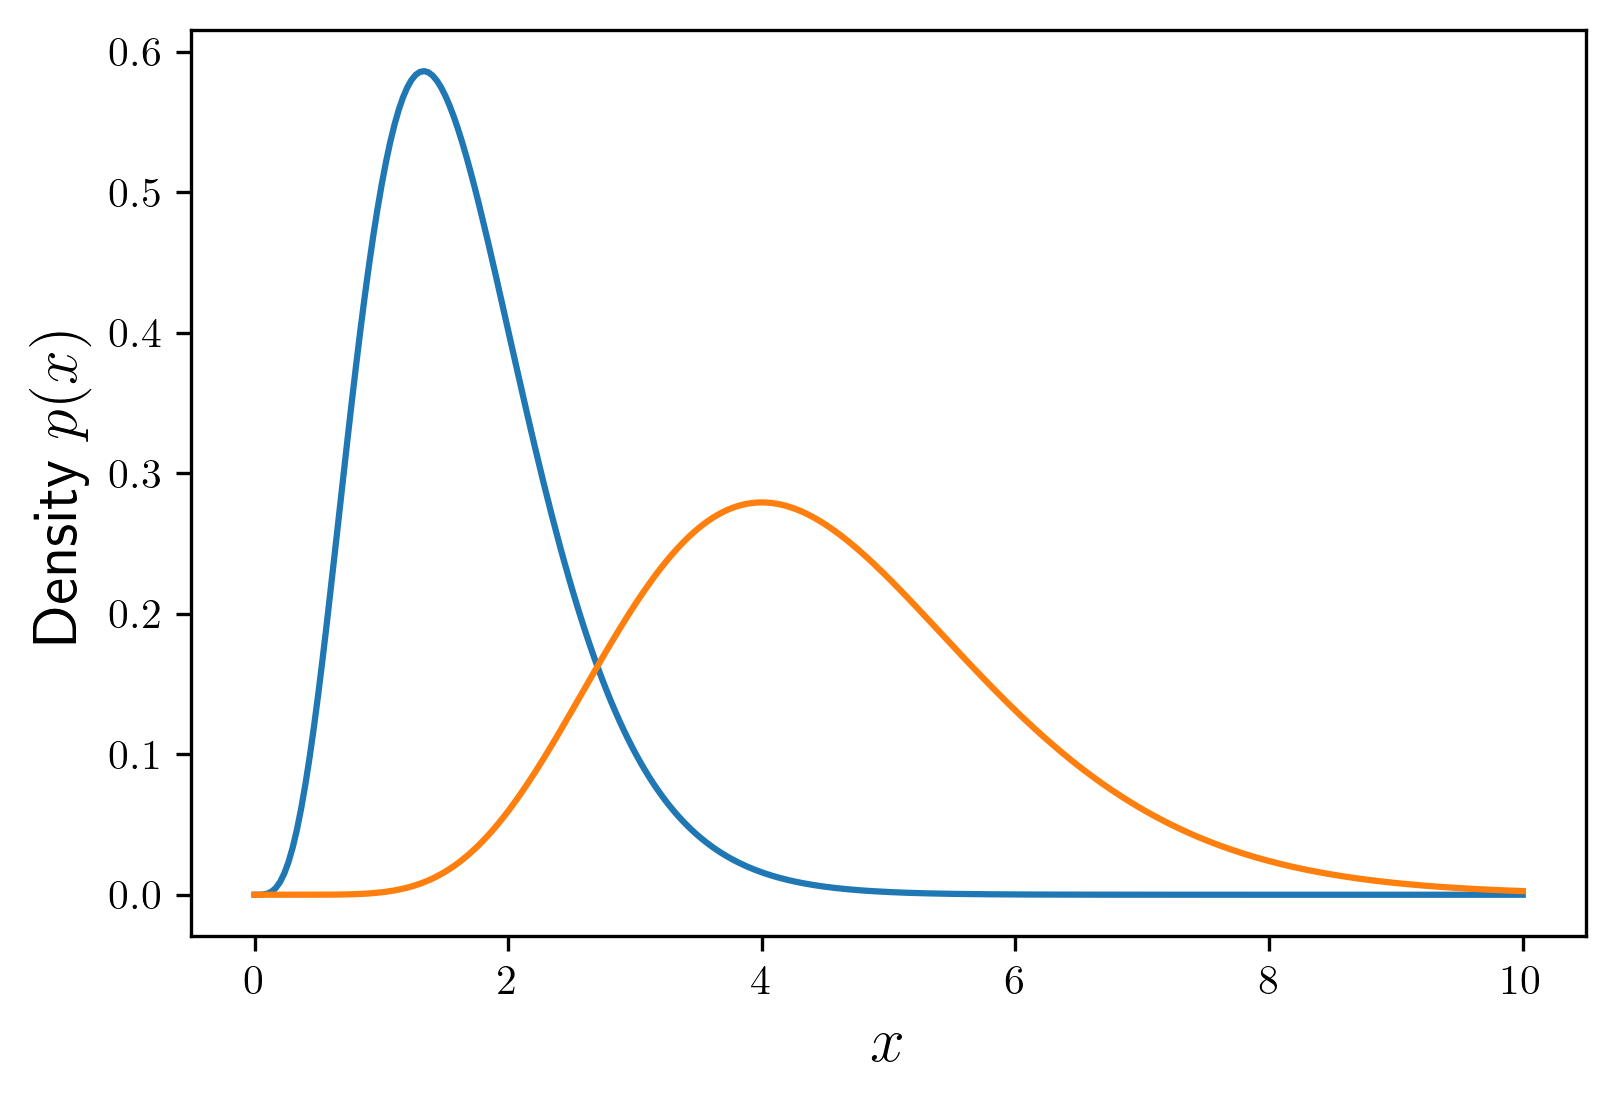
\includegraphics[width=0.8\textwidth]{./figures/stochastic_domination_pdf.png}
	\caption{Example of stochastic domination - PDFs}
\end{figure}
\begin{figure}[h]
	\centering
	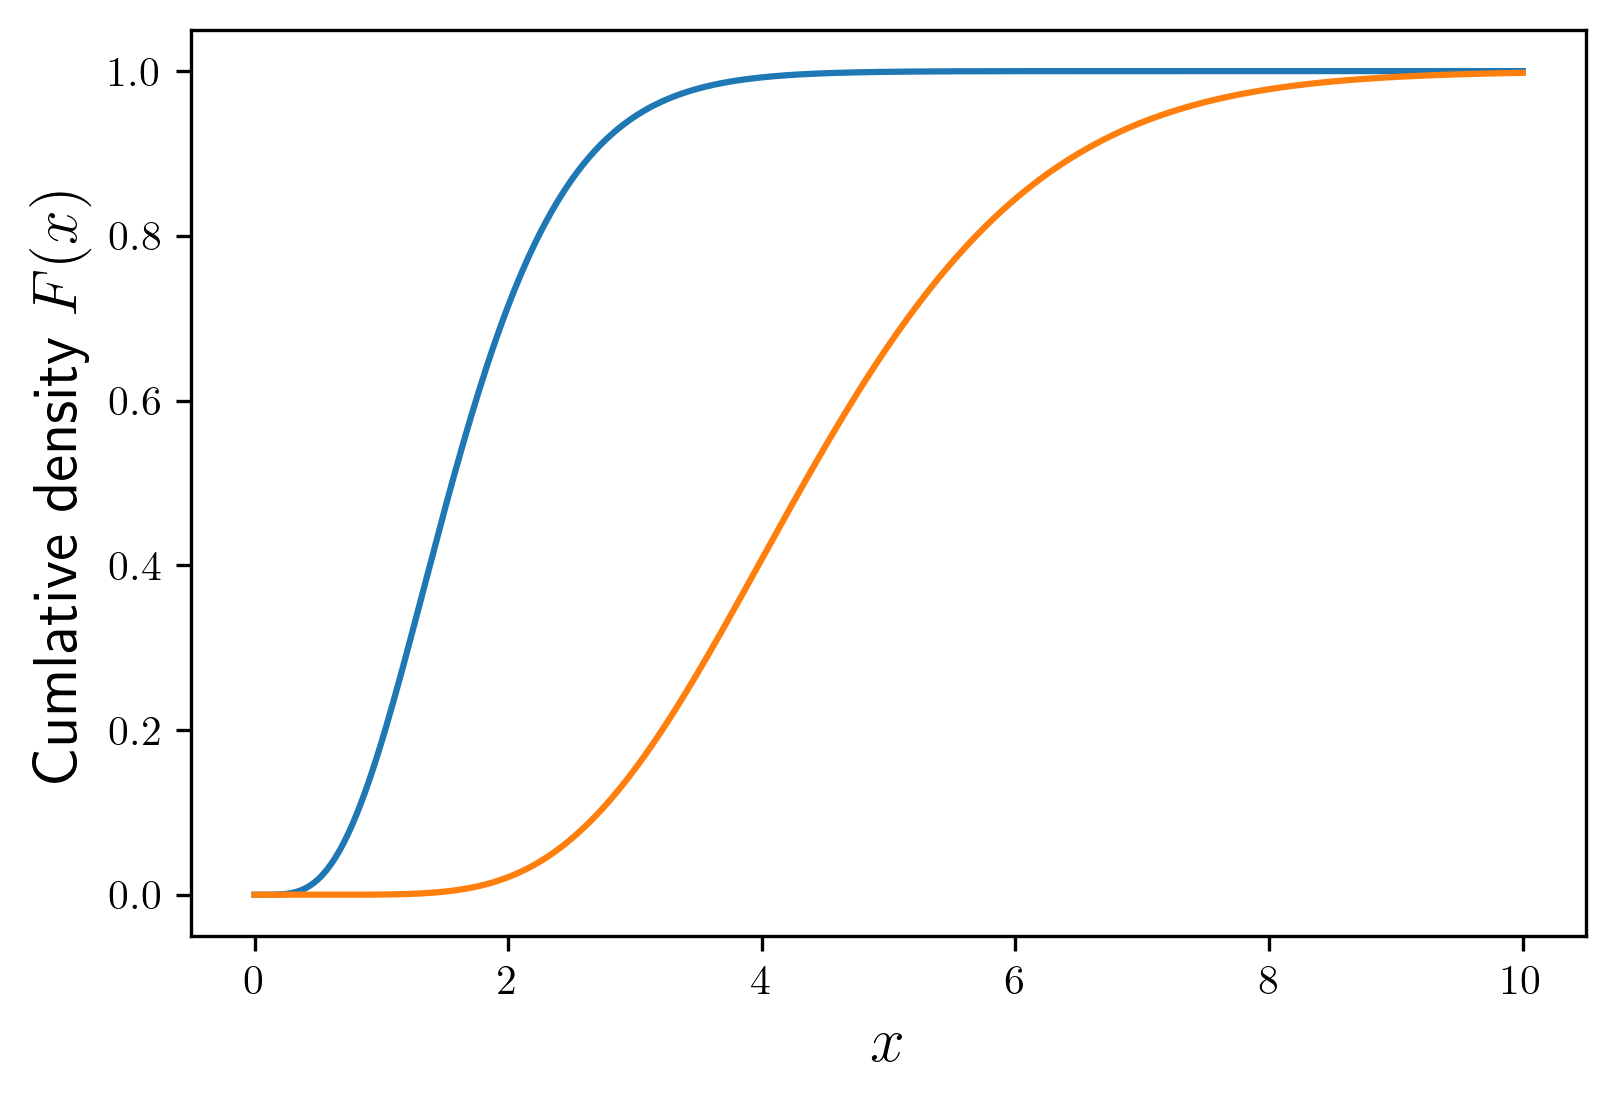
\includegraphics[width=0.8\textwidth]{./figures/stochastic_domination_cdf.png}
	\caption{Example of stochastic domination - CDFs}
\end{figure}

\begin{definition} % TODO: Check definition
	Coupling

	\noindent
	A  coupling of the real random variables $X$ and $Y$ is a joint random variable $(\tilde{X}, \tilde{Y})$ such that the marginal distribution of $\tilde{X}$ is the same as $X$, and the marginal distribution of $\tilde{Y}$ is the same as $Y$.
\end{definition}

% TODO: when allowed different samples spaces, interpreation

\begin{theorem}\label{theorem:couplingDomination}
	The real random variable $X$ is stochastically dominated by the real random variable $Y$ if and only if there exists a coupling $(\tilde{X}, \tilde{Y})$ of $X$ and $Y$ such that
	$$
		\mathbb{P}(\tilde{Y} \geq \tilde{X}) = 1
	$$
\end{theorem}

\begin{proof}
	We prove the forwards implication. Suppose there exists a coupling $(\tilde{X}, \tilde{Y})$ of $X$ and $Y$ such that $\mathbb{P}(\tilde{Y} \geq \tilde{X}) = 1$. Then for all $x \in \mathbb{R}$
	\begin{align*}
		\mathbb{P}(X \geq x) &= \mathbb{P}(\tilde{X} \geq x) & \text{since } \tilde{X} \stackrel{d}{=} X \\
		&\leq \mathbb{P}(\tilde{Y} \geq x) & \text{since with probability 1, } \tilde{Y} \geq \tilde{X} \\
		&= \mathbb{P}(Y \geq x) & \text{since } \tilde{Y} \stackrel{d}{=} Y 
	\end{align*}

	We omit the proof for the reverse implication as we only use the forwards implication. For the proof of the reverse implication, see \cite{coupling}.
\end{proof}

% TODO, introduce equal in distribution in coupling definition

We omit the proof, but refer the reader to \cite{coupling} for details.

\begin{theorem}
	Let $0 < \lambda < \mu$. If $X \sim \text{Poisson}(\lambda)$ and $Y \sim \text{Poisson}(\mu)$ are independent random variables, then $X \preceq Y$. 
\end{theorem}

\begin{proof}
	Let $\tilde{X} \sim \text{Poisson}(\lambda)$, $\tilde{Z} \sim \text{Poisson}(\mu - \lambda)$ be independent random variables. Hence, we have that $\tilde{Y} := \tilde{X} + \tilde{Z} \sim \text{Poisson}(\mu)$. Note that since $\tilde{Z} \geq 0$, the value taken by $\tilde{Y}$ is always at least the value taken by $\tilde{X}$. Since we have found a coupling $(\tilde{X}, \tilde{Y})$ of $X$ and $Y$ where $\mathbb{P}(\tilde{Y} \geq \tilde{X}) = 1$, by Theorem \ref{theorem:couplingDomination}, $X \preceq Y$.
\end{proof}

\begin{theorem}
	Let $X \sim \text{Binomial}(n_1, p)$ and $Y \sim \text{Binomial}(n_2, p)$ with $n_1 < n_2$. Then $X$ is stochastically dominated by $Y$.
\end{theorem}

\begin{proof}
	Let $X_1, \dots, X_{n_2}$ be an iid sequence of Bernoulli random variables where $\mathbb{P}(X_i = 1) = p$. We observe that $\tilde{X} := \sum_{i=1}^{n_1} X_i \sim \text{Binomial}(n_1, p)$ and $\tilde{Y} := \sum_{i=1}^{n_2} X_i \sim \text{Binomial}(n_2, p)$. Since $X_i \geq 0$ for all $i$, and $\tilde{Y} = \tilde{X} + X_{n_1 + 1} + \dots + X_{n_2}$, we have that $\tilde{X} \leq \tilde{Y}$. Hence, by Theorem \ref{theorem:couplingDomination}, $X \preceq Y$.
\end{proof}

% TODO: Discuss implications for async rumour spreading - interpreting poission process as exponential clock, not interested in value of the process

